\tikzstyle{startstop} = [rectangle, rounded corners, minimum width=10cm, minimum height=1.5cm,text centered, draw=black, fill=green!20]
\begin{center}
	\begin{tikzpicture}
	\node (start) [startstop] {\bfseries \text{ÔN TẬP BÀI 1 VÀ BÀI 2}};
	\end{tikzpicture}
\end{center}
\setcounter{section}{0}
\section{Câu trắc nghiệm nhiều phương án lựa chọn}
%\textit{Thí sinh trả lời từ câu 1 đến câu 18. Mỗi câu hỏi thí sinh chọn một phương án}
\setcounter{ex}{0}
\Opensolutionfile{ans}[ans/G11BT1+2TN]
% ===================================================================
\begin{ex}
	Chuyển động nào sau đây \textbf{không} được gọi là dao động cơ?
	\choice
	{Chuyển động lên xuống của piston trong cylanh của động cơ}
	{Chuyển động qua lại của con lắc đồng hồ}
	{\True Chuyển động của xe ô tô trên đường}
	{Chuyển động của dây đàn khi được gảy}
	\loigiai{}
\end{ex}
% ===================================================================
\begin{ex}
	Dao động tuần hoàn là dao động có đặc điểm
	\choice
	{vật trở lại vị trí cũ sau những khoảng thời gian bằng nhau}
	{vật có hướng chuyển động như cũ sau những khoảng thời gian bằng nhau}
	{\True vật trở lại vị trí cũ theo hướng cũ sau những khoảng thời gian bằng nhau}
	{vật trở lại vị trí cũ theo hướng cũ sau những khoảng thời gian bất kì}
	\loigiai{}
\end{ex}
% ===================================================================
\begin{ex}
Trong các phương trình sau, phương trình nào biểu diễn dao động điều hoà?
	\choice
	{$x=2\tan\left(2\pi t\right)$ cm}
	{$x=3t\cos\left(5\pi t\right)$ cm}
	{$x=\cos \left(0,5\pi t^{3}\right)$ cm}
	{\True $x=\cos\left(100\pi t\right)$ cm}
	\loigiai{}
\end{ex}
% ===================================================================
\begin{ex}
	Pha ban đầu của dao động điều hoà phụ thuộc vào
	\choice
	{\True cách chọn gốc thời gian}
	{biên độ của con lắc}
	{cách kích thích dao động}
	{cấu tạo con lắc lò xo}
	\loigiai{}
\end{ex}
% ===================================================================
\begin{ex}
	Đồ thị li độ - thời gian của một dao động điều hoà sẽ có dạng
	\choice
	{\True một đường hình sin}
	{một đoạn thẳng}
	{một đường tròn}
	{một đường thẳng}
	\loigiai{}
\end{ex}
% ===================================================================
\begin{ex}
Trong dao động điều hoà, đại lượng nào sau đây \textbf{không phải} là hằng số?	
	\choice
	{\True Li độ}
	{Biên độ}
	{Pha ban đầu}
	{Tần số góc}
	\loigiai{}
\end{ex}
% ===================================================================
\begin{ex}
Khi một vật dao động điều hoà, biên độ $A$ là	
	\choice
	{độ dịch chuyển từ vị trí cân bằng đến vị trí của vật}
	{\True độ dịch chuyển cực đại của vật tính từ vị trí cân bằng}
	{độ dịch chuyển cực đại của vật tính từ vị trí biên}
	{độ dịch chuyển của vật tính từ vị trí biên}
	\loigiai{}
\end{ex}
% ===================================================================
\begin{ex}
Trong dao động điều hoà, tần số $f$ và chu kì $T$	
	\choice
	{$f=\dfrac{1}{T^2}$}
	{$f^2=\dfrac{1}{T}$}
	{$f=T$}
	{\True $f=\dfrac{1}{T}$}
	\loigiai{}
\end{ex}
% ===================================================================
\begin{ex}
	Đại lượng nào sau đây \textbf{không phải} là một trong các đại lượng đặc trưng của một dao động điều hoà?
	\choice
	{Chu kì}
	{Tần số góc}
	{\True Pha ban đầu}
	{Tần số}
	\loigiai{}
\end{ex}
% ===================================================================
\begin{ex}
	Trong dao động điều hoà, tần số góc $\omega$ và chu kì $T$ liên hệ với nhau theo công thức 
	\choice
	{$\omega =2\pi T$}
	{\True $\omega=\dfrac{2\pi}{T}$}
	{$\omega=\dfrac{T}{2\pi}$}
	{$\omega=\dfrac{\pi}{T}$}
	\loigiai{}
\end{ex}
% ===================================================================
\begin{ex}
Các đặc trưng cơ bản của dao động điều hoà là	
	\choice
	{\True biên độ và tần số}
	{tần số và pha ban đầu}
	{bước sóng và biên độ}
	{vận tốc và gia tốc}
	\loigiai{}
\end{ex}
% ===================================================================
\begin{ex}
Để biết một vật dao động điều hoà ở đâu và đi về phía nào khi bắt đầu dao động người ta dựa vào	
	\choice
	{chu kì}
	{\True pha ban đầu}
	{li độ}
	{biên độ}
	\loigiai{}
\end{ex}
% ===================================================================
\begin{ex}
	Chu kì trong dao động điều hoà là khoảng thời gian
	\choice
	{\True để vật thực hiện một dao động}
	{để vật trở lại vị trí cũ}
	{giữa hai lần liên tiếp vật đổi chiều chuyển động}
	{giữa hai lần liên tiếp vật đi qua vị trí cân bằng}
	\loigiai{}
\end{ex}
% ===================================================================
\begin{ex}
Số dao động mà vật thực hiện được trong một giây gọi là	
	\choice
	{tần số góc}
	{\True tần số}
	{chu kì}
	{pha dao động}
	\loigiai{}
\end{ex}
% ===================================================================
\begin{ex}
	Đơn vị của tần số góc là
	\choice
	{giây $\left(\si{\second}\right)$}
	{héc $\si{\hertz}$}
	{\True radian/giây $\si{\radian/\second}$}
	{radian $\left(\si{\radian}\right)$}
	\loigiai{}
\end{ex}
% ===================================================================
\begin{ex}
	Một vật dao động điều hoà với phương trình $x=\xsi{6\cos\left(\pi t-\dfrac{\pi}{6}\right)}{\centi\meter}$, pha dao động tại thời điểm $t=\SI{2}{\second}$ là
	\choice
	{\True $\xsi{\dfrac{11\pi}{6}}{\radian}$}
	{$\xsi{-\dfrac{\pi}{6}}{\radian}$}
	{$\xsi{\dfrac{13\pi}{6}}{\radian}$}
{$\xsi{2\pi}{\radian}$}
	\loigiai{}
\end{ex}
% ===================================================================
\begin{ex}
	Đồ thị li độ - thời gian của một vật dao động điều hoà được mô tả như hình vẽ. Biên độ dao động của vật là
	\begin{center}
		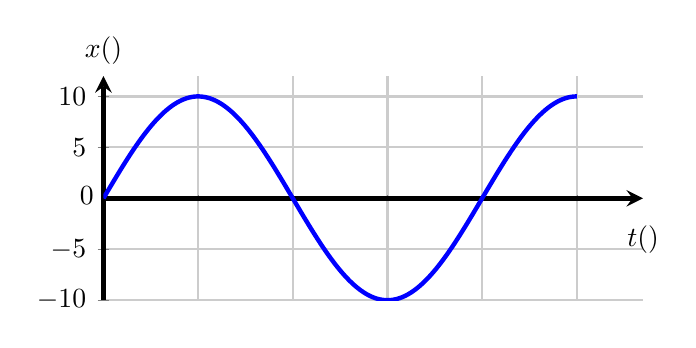
\begin{tikzpicture}  
			\begin{axis}[  ultra thick,
				xmin=0,  
				xmax=5.7, 
				ymin=-10,  
				ymax=12, 
				xtick={0,1,...,5},
				ytick={-10,-5,...,10},
				xticklabels=\empty,
%				minor x tick num=0,
%				minor y tick num=1,
				samples=300,
				axis lines=middle, 
				grid style={step=1, color=gray!20!white},
				grid=both,
				major grid style={line width=0.8pt,gray!40!white},
				xlabel=$\xsi{t}{\left(\second\right)}$, 
				ylabel=$\xsi{x}{\left(\si{\centi\meter}\right)}$, 
				every axis y label/.style={at=(current axis.above origin),anchor=south},  
				every axis x label/.style={at=(current axis.right of origin),anchor=east, below=1.5cm}, yscale=0.5 ]  
				\addplot [ultra thick, blue, smooth, domain=0:5] {10*cos(deg(pi*x/2-pi/2))}; 
			\end{axis}
		\node[label={[left]90:0}] at (0,1.2){};  
		\end{tikzpicture}
	\end{center}
	\choice
	{$\SI{20}{\centi\meter}$}
	{\True $\SI{10}{\centi\meter}$}
	{$\SI{5}{\centi\meter}$}
	{$\SI{30}{\centi\meter}$}
	\loigiai{}
\end{ex}
% ===================================================================
\begin{ex}
Một vật dao động điều hoà có đồ thị li độ - thời gian được mô tả như hình bên. Chu kì dao động của vật là	
	\begin{center}
		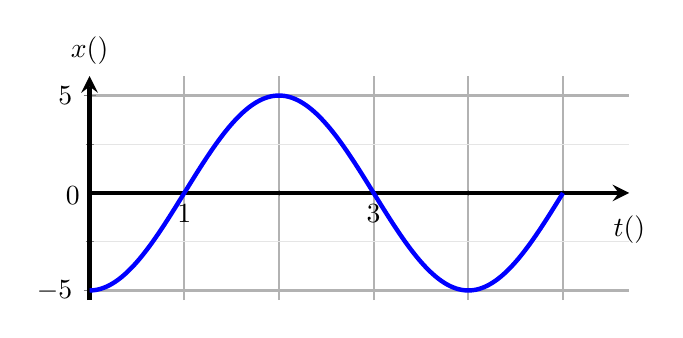
\begin{tikzpicture}  
			\begin{axis}[  ultra thick,
				xmin=0,  
				xmax=5.7, 
				ymin=-5.5,  
				ymax=6, 
				xtick={0,1,...,5},
				ytick={-5,0,5},
				xticklabels=\empty,
				%				minor x tick num=0,
							minor y tick num=1,
				samples=300,
				axis lines=middle, 
				grid style={step=1, color=gray!20!white},
				grid=both,
				major grid style={line width=0.8pt,gray!60!white},
				xlabel=$\xsi{t}{\left(\second\right)}$, 
				ylabel=$\xsi{x}{\left(\si{\centi\meter}\right)}$, 
				every axis y label/.style={at=(current axis.above origin),anchor=south},  
				every axis x label/.style={at=(current axis.right of origin),anchor=east, below=1.5cm}, yscale=0.5 ]  
				\addplot [ultra thick, blue, smooth, domain=0:5] {5*cos(deg(pi*x/2-pi))}; 
				\node at (axis cs:1,0) [below] {1};
				\node at (axis cs:3,0) [below] {3};
			\end{axis}
			\node[label={[left]90:0}] at (0,1.2){};  
		\end{tikzpicture}
	\end{center}
	\choice
	{$\SI{1}{\second}$}
	{$\SI{2}{\second}$}
	{\True $\SI{4}{\second}$}
	{$\SI{3}{\second}$}
	\loigiai{}
\end{ex}
% ===================================================================
\begin{ex}
Một vật dao động điều hoà với phương trình li độ $x=\xsi{4\cos\left(4\pi t-\dfrac{\pi}{4}\right)}{\centi\meter}$. Chu kì dao động của vật là	
	\choice
	{$\xsi{4\pi}{\second}$}
	{$\SI{2}{\second}$}
	{\True $\SI{0.5}{\second}$}
	{$\xsi{2\pi}{\second}$}
	\loigiai{}
\end{ex}
% ===================================================================
\begin{ex}
Một vật dao động điều hoà, trong thời gian 1 phút vật thực hiện được 20 dao động. Tần số dao động của vật là	
	\choice
	{\True $\xsi{\dfrac{1}{3}}{\hertz}$}
	{$\SI{3}{\hertz}$}
	{$\SI{120}{\hertz}$}
	{$\SI{20}{\hertz}$}
	\loigiai{}
\end{ex}
% ===================================================================
\begin{ex}
Cho vật dao động điều hoà có đồ thị li độ - thời gian được mô tả như hình bên. Thời gian giữa hai lần liên tiếp vật đi qua vị trí cân bằng là
	\begin{center}
		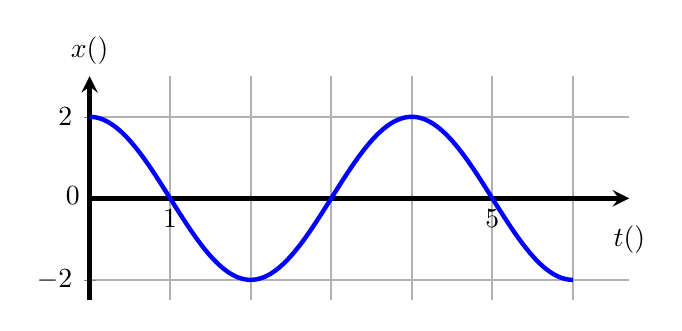
\begin{tikzpicture}  
			\begin{axis}[  ultra thick,
				xmin=0,  
				xmax=6.7, 
				ymin=-2.5,  
				ymax=3, 
				xtick={0,1,...,6},
				ytick={-2,0,2},
				xticklabels=\empty,
				%				minor x tick num=0,
				%minor y tick num=1,
				samples=300,
				axis lines=middle, 
				grid style={step=1, color=gray!20!white},
				grid=both,
				major grid style={line width=0.8pt,gray!60!white},
				xlabel=$\xsi{t}{\left(\second\right)}$, 
				ylabel=$\xsi{x}{\left(\si{\centi\meter}\right)}$, 
				every axis y label/.style={at=(current axis.above origin),anchor=south},  
				every axis x label/.style={at=(current axis.right of origin),anchor=east, below=1.5cm}, yscale=0.5 ]  
				\addplot [ultra thick, blue, smooth, domain=0:6] {2*cos(deg(pi*x/2))}; 
				\node at (axis cs:1,0) [below] {1};
				\node at (axis cs:5,0) [below] {5};
			\end{axis}
			\node[label={[left]90:0}] at (0,1.2){};  
		\end{tikzpicture}
	\end{center}
	\choice
	{$\SI{1}{\second}$}
	{$\SI{5}{\second}$}
	{$\SI{4}{\second}$}
	{\True $\SI{2}{\second}$}
	\loigiai{}
\end{ex}
% ===================================================================
\begin{ex}
	Cho hai vật dao động điều hoà với các phương trình li độ:
	$$x_1=\xsi{5\cos\left(3\pi t+\dfrac{\pi}{3}\right)}{\centi\meter}\quad \text{và}\quad x_2=\xsi{4\cos\left(3\pi t-\dfrac{\pi}{6}\right)}{\centi\meter}.$$ Độ lệch pha của hai dao động này là
	\choice
	{$\xsi{\dfrac{\pi}{3}}{\radian}$}
	{\True $\xsi{\dfrac{\pi}{2}}{\radian}$}
	{$\xsi{\dfrac{\pi}{6}}{\radian}$}
	{$\xsi{\dfrac{2\pi}{3}}{\radian}$}
	\loigiai{}
\end{ex}
% ===================================================================
\begin{ex}
Cho hai vật dao động điều hoà	cùng chu kì có đồ thị li độ - thời gian được mô tả như hình bên. Độ lệch pha giữa hai dao động là
\begin{center}
	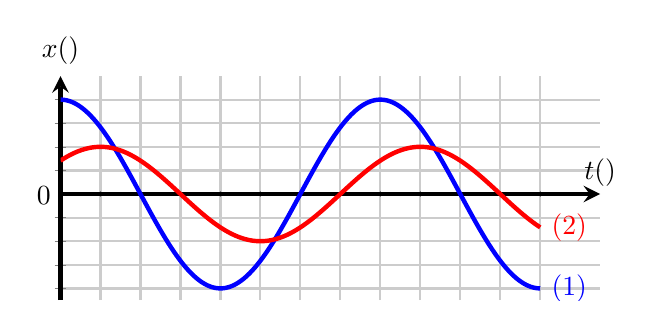
\begin{tikzpicture}  
		\begin{axis}[  ultra thick,
			xmin=0,  
			xmax=13.5, 
			ymin=-4.5,  
			ymax=5, 
			xtick={0,1,...,12},
			ytick={-4,-3,...,4},
			xticklabels=\empty,
			yticklabels=\empty,
			%				minor x tick num=0,
			%minor y tick num=1,
			samples=300,
			axis lines=middle, 
			grid style={step=1, color=gray!20!white},
			grid=both,
			major grid style={line width=0.8pt,gray!40!white},
			xlabel=$\xsi{t}{\left(\second\right)}$, 
			ylabel=$\xsi{x}{\left(\si{\centi\meter}\right)}$, 
			every axis y label/.style={at=(current axis.above origin),anchor=south},  
			every axis x label/.style={at=(current axis.right of origin),anchor=east, below=0.75cm}, yscale=0.5 ]  
			\addplot [ultra thick, blue, smooth, domain=0:12] {4*cos(deg(pi*x/4))} node [right] {(1)}; 
			\addplot [ultra thick, red, smooth, domain=0:12] {2*cos(deg(pi*x/4-pi/4))} node [right] {(2)};
		\end{axis}
		\node[label={[left]90:0}] at (0,1.2){};  
	\end{tikzpicture}
\end{center}
	\choice
	{\True $\xsi{\dfrac{\pi}{4}}{\radian}$}
	{$\xsi{\dfrac{\pi}{2}}{\radian}$}
	{$\xsi{2\pi}{\radian}$}
	{$\SI{0}{\radian}$}
	\loigiai{}
\end{ex}
% ===================================================================
\begin{ex}
Cho hai con lắc lò xo cùng dao động điều hoà có cùng tần số và cùng biên độ với phương trình li độ của con lắc thứ nhất $x_1=\xsi{4\cos\left(4\pi t+\dfrac{2\pi}{3}\right)}{\centi\meter}$. Biết thời gian con lắc thứ hai có cùng trạng thái với con lắc thứ nhất là muộn hơn $\SI{0.1}{\second}$. Phương trình dao động của con lắc thứ hai là	
	\choice
	{$x_2=\xsi{4\cos\left(4\pi t-\dfrac{\pi}{5}\right)}{\centi\meter}$}
	{$x_2=\xsi{4\cos\left(4\pi t+\dfrac{2\pi}{5}\right)}{\centi\meter}$}
	{$x_2=\xsi{4\cos\left(4\pi t-\dfrac{2\pi}{15}\right)}{\centi\meter}$}
	{$x_2=\xsi{4\cos\left(4\pi t+\dfrac{4\pi}{15}\right)}{\centi\meter}$}
	\loigiai{}
\end{ex}
% ===================================================================
\begin{ex}
	Cho hai vật dao động điều hoà cùng chu kì có đồ thị li độ - thời gian được mô tả như hình bên. Độ lệch pha giữa hai dao động là
	\begin{center}
		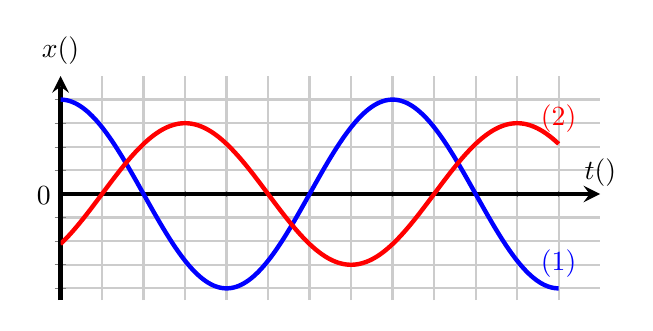
\begin{tikzpicture}  
			\begin{axis}[  ultra thick,
				xmin=0,  
				xmax=13, 
				ymin=-4.5,  
				ymax=5, 
				xtick={0,1,...,12},
				ytick={-4,-3,...,4},
				xticklabels=\empty,
				yticklabels=\empty,
				%				minor x tick num=0,
				%minor y tick num=1,
				samples=300,
				axis lines=middle, 
				grid style={step=1, color=gray!20!white},
				grid=both,
				major grid style={line width=0.8pt,gray!40!white},
				xlabel=$\xsi{t}{\left(\second\right)}$, 
				ylabel=$\xsi{x}{\left(\si{\centi\meter}\right)}$, 
				every axis y label/.style={at=(current axis.above origin),anchor=south},  
				every axis x label/.style={at=(current axis.right of origin),anchor=east, below=0.75cm}, yscale=0.5 ]  
				\addplot [ultra thick, blue, smooth, domain=0:12] {4*cos(deg(pi*x/4))} node [above] {(1)}; 
				\addplot [ultra thick, red, smooth, domain=0:12] {3*cos(deg(pi*x/4-3*pi/4))} node [above] {(2)};
			\end{axis}
			\node[label={[left]90:0}] at (0,1.2){};  
		\end{tikzpicture}
	\end{center}
	\choice
	{$\xsi{\dfrac{\pi}{4}}{\radian}$}
	{\True $\xsi{\dfrac{3\pi}{4}}{\radian}$}
	{$\xsi{2\pi}{\radian}$}
	{$\xsi{\dfrac{5\pi}{6}}{\radian}$}
	\loigiai{}
\end{ex}
\Closesolutionfile{ans}
\section{Tự luận}
\setcounter{ex}{0}
% ===================================================================
\begin{ex}
	Một vật dao động điều hoà có phương trình li độ $x=\xsi{2\cos\left(\pi t-\dfrac{\pi}{6}\right)}{\centi\meter}$, trong đó $t$ tính bằng giây. Trong $\SI{12}{\second}$ vật thực hiện được bao nhiêu dao động?
	\loigiai{$N=\dfrac{\Delta t}{T}=6$.}
\end{ex}
% ===================================================================
\begin{ex}
Xác định biên độ, chu kì, tần số và pha ban đầu của các dao động điều hoà sau:
\begin{enumerate}[label=\alph*)]
	\item $x=\xsi{5\cos\left(2\pi t-\dfrac{\pi}{2}\right)}{\centi\meter}$.
	\item $x=\xsi{-5\cos\left(\pi t-\dfrac{\pi}{6}\right)}{\centi\meter}$.
\end{enumerate}
	\loigiai{}
\end{ex}
% ===================================================================
\begin{ex}
	Một vật dao động điều hoà trên đoạn thẳng có chiều dài $\SI{4}{\centi\meter}$, vật thực hiện được 100 dao động trong $\SI{20}{\second}$. Tính biên độ, chu kì, tần số và tần số góc của dao động.
	\loigiai{}
\end{ex}
% ===================================================================
\begin{ex}
	Một vật dao động điều hoà với phương trình li độ $x=\xsi{5\cos\left(4\pi t+\dfrac{2\pi}{3}\right)}{\centi\meter}$, trong đó $t$ tính bằng giây.
	\begin{enumerate}[label=\alph*)]
		\item Xác định biên độ, tần số góc và pha ban đầu của dao động.
		\item Xác định chiều dài quỹ đạo của vật dao động.
		\item Xác định pha của dao động và li độ của vật tại các thời điểm $\SI{0.25}{\second}$ và $\SI{0.5}{\second}$.
	\end{enumerate}
	\loigiai{}
\end{ex}
% ===================================================================
\begin{ex}
	Một vật dao động điều hoà với phương trình li độ $x=\xsi{6\cos\left(3\pi t+\dfrac{\pi}{3}\right)}{\centi\meter}$ trong đó $t$ tính bằng giây. Lúc $t=\SI{2.0}{\second}$ thì các đại lượng sau đây có giá trị bằng bao nhiêu?
	\begin{enumerate}[label=\alph*)]
		\item Pha dao động.
		\item Li độ.
		\item Chu kì.
		\item Tần số.
	\end{enumerate}
	\loigiai{}
\end{ex}
% ===================================================================
\begin{ex}
	Đồ thị li độ - thời gian của hai vật dao động điều hoà $x_1\left(t\right)$ và $x_2\left(t\right)$ như hình vẽ. Xác định độ lệch pha giữa dao động của vật 1 so với dao động của vật 2.
	\begin{center}
		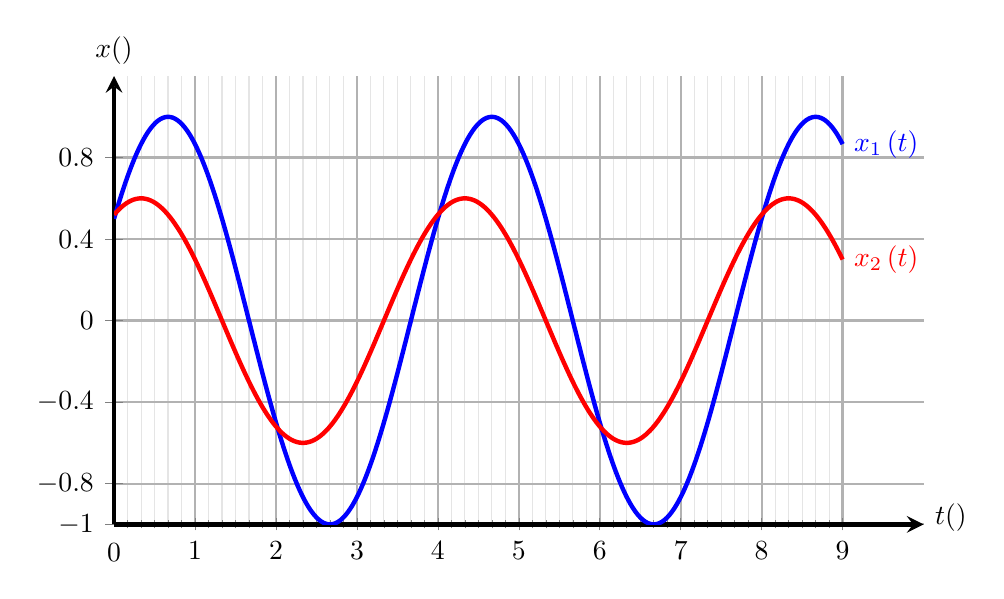
\begin{tikzpicture}  
			\begin{axis}[  ultra thick,
				xmin=0,  
				xmax=10, 
				ymin=-1,  
				ymax=1.2, 
				xtick={0,1,...,9},
				ytick={-1,-0.8,-0.4,0,0.4,0.8},
				minor x tick num=5,
				minor y tick num=1,
				samples=300,
				axis lines=middle, 
				axis x line shift={1},
				grid style={step=1, color=gray!20!white},
				grid=both,
				major grid style={line width=0.8pt,gray!60!white},
				xlabel=$\xsi{t}{\left(\second\right)}$, 
				ylabel=$\xsi{x}{\left(\si{\centi\meter}\right)}$, 
				every axis y label/.style={at=(current axis.above origin),anchor=south},  
				every axis x label/.style={at=(current axis.right of origin),below=2.5cm,anchor=west}, xscale=1.5]  
				\addplot [ultra thick, blue, smooth, domain=0:9] {1*cos(deg(pi*x/2-pi/3))} node [right] {$x_1\left(t\right)$}; 
				\addplot [ultra thick, red, smooth, domain=0:9] {0.6*cos(deg(pi*x/2-pi/6))} node [right] {$x_2\left(t\right)$};
			\end{axis}
		\node[label={[below]90:0}] at (0,-0.25){};
		\end{tikzpicture}
	\end{center}
	\loigiai{$\Delta \varphi=\xsi{\dfrac{\pi}{6}}{\radian}$.}
\end{ex}
% ===================================================================
\begin{ex}
	Đồ thị li độ - thời gian của 2 vật dao động điều hoà được thể hiện như hình vẽ.
		\begin{center}
		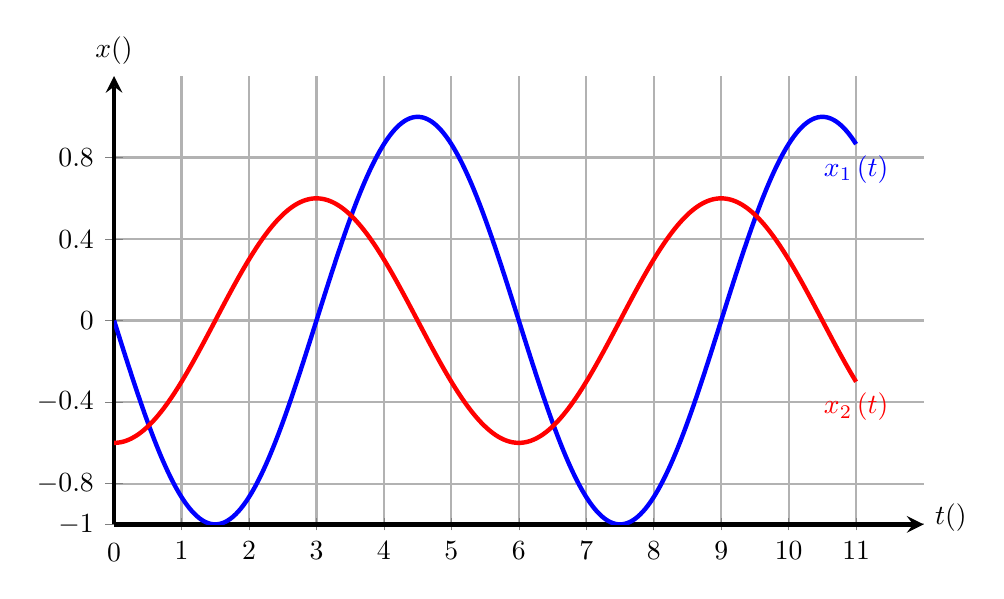
\begin{tikzpicture}  
			\begin{axis}[  ultra thick,
				xmin=0,  
				xmax=12, 
				ymin=-1,  
				ymax=1.2, 
				xtick={0,1,...,11},
				ytick={-1,-0.8,-0.4,0,0.4,0.8},
%				minor x tick num=5,
%				minor y tick num=1,
				samples=300,
				axis lines=middle, 
				axis x line shift={1},
				grid style={step=1, color=gray!20!white},
				grid=both,
				major grid style={line width=0.8pt,gray!60!white},
				xlabel=$\xsi{t}{\left(\second\right)}$, 
				ylabel=$\xsi{x}{\left(\si{\centi\meter}\right)}$, 
				every axis y label/.style={at=(current axis.above origin),anchor=south},  
				every axis x label/.style={at=(current axis.right of origin),below=2.5cm,anchor=west}, xscale=1.5]  
				\addplot [ultra thick, blue, smooth, domain=0:11] {1*cos(deg(pi*x/3+pi/2))} node [below] {$x_1\left(t\right)$}; 
				\addplot [ultra thick, red, smooth, domain=0:11] {0.6*cos(deg(pi*x/3-pi))} node [below] {$x_2\left(t\right)$};
			\end{axis}
			\node[label={[below]90:0}] at (0,-0.25){};
		\end{tikzpicture}
	\end{center}
	\begin{enumerate}[label=\alph*)]
		\item Xác định tần số của mỗi dao động.
		\item Cho biết dao động của vật 1 hay dao động của vật 2 đạt cực đại trước? Giải thích.
		\item Xác định độ lệch pha giữa dao động của vật 1 và dao động của vật 2.
	\end{enumerate}
	\loigiai{}
\end{ex}
